\section{Fitting discrete distributions}\label{sec:discrete-fit}

Often interest is focused on how closely such data follow a
particular distribution, such as the Poisson, binomial, or geometric
distribution.  Usually this is examined with a classical (Pearson)
goodness-of-fit chi-square test,
\glosstex{chi-square test}

\begin{equation}\label{eq:chi2}
  \chi^2 = \sum_{k=1}^K \:
  \frac{{ ( n_k - N \hat{p}_k ) }^2}
  { N \hat{p}_k }  \sim \chi^2_{( K-s-1 )}
  \comma
\end{equation}
where there are $K$ frequency classes, 
$s$ parameters have been estimated from the data and
\(\hat{p}_k\) is the estimated probability of each basic count,
under the null hypothesis that the data follows the chosen distribution.
An alternative test statistic is the likelihood-ratio $G^2$
statistic,
\begin{equation}\label{eq:g2}
 G^2 = \sum_{k=1}^K \: n_k \log ( n_k / N \hat{p}_k )
 \comma
\end{equation}
when the $\hat{p}_k$ are estimated by maximum likelihood,
which also has an asymptotic $\chi^2_{(K - s - 1)}$ distribution.
``Asymptotic'' means that these are large sample tests.
A common rule of thumb is that all expected frequencies
should exceed one and that fewer than 20\% should be less than 5.

For the horse kick data, the mean is 122/200 = .610, and calculation
of Poisson probabilities (\texttt{PHAT}), expected frequencies, and
contributions to \(\chi^2\) \eqref{eq:chi2} are shown below.
\ixd{deaths by horsekick}

\begin{center}
\begin{alltt}
 k     nk      p        phat         exp     chisq

 0    109    0.545    0.54335    108.670    0.00100
 1     65    0.325    0.33144     66.289    0.02506
 2     22    0.110    0.10109     20.218    0.15705
 3      3    0.015    0.02056      4.111    0.30025
 4      1    0.005    0.00313      0.627    0.22201
      ===                        =======    =======
      200                        199.915    0.70537 \(\sim \chi\sp2 (3)\)
\end{alltt}
\end{center}

In this case the \(\chi^2\) shows an exceptionally good (perhaps unreasonably
good?) fit.  In the word frequency example
(\exref{ex:madison1}), the fit of the Poisson
turns out not to be close at all.  However, even a close fit may show
something interesting, if we know how to look; conversely, it is
useful to know why or where the data differ from a chosen model.

\subsection{The \macro{GOODFIT}}
The \macro{GOODFIT} (see \macref{mac:goodfit}) carries out Pearson \chisq{} and \LR{} goodness-of fit tests
for the uniform, binomial, Poisson, negative binomial,
 logarithmic series, and geometric distributions,
as well as any discrete (multinomial) distribution whose probabilities you can specify.
The data may consist either of individual observations on a single
variable, or a grouped frequency distribution in the form
shown in \tabref{tab:horskick}.
The parameter(s) of the distribution may be specified as constants
or may be estimated from the data.

\begin{comment}  %%% begin stuff deleted
The macro is used as follows%
\footnote{In subsequent descriptions of macros in the text
we simply give references to the documentation provided in Appendix \ref{ch:macros} and provide examples of usage.}%
:
\aunote{Should we take this out?}
\begin{listing}
\%goodfit(data=\emph{SASdatasetname},
   var=\emph{variablename},
   freq=\emph{variablename},
   dist=\emph{distribution},
   parm=\emph{parameters},
   sumat=\emph{value},
   format=\emph{SASformat},
   out=\emph{outputdatasetname},
   outstat=\emph{statisticsdatasetname});
\end{listing}
\end{comment}  
The macro parameters are described in \macref{mac:goodfit}.
We illustrate its use in \exref{ex:weldon} and \exref{ex:federalist} below.

\begin{Example}[weldon]{Weldon's dice}
The data from \tabref{tab:dice}
can be fit to a binomial distribution as shown below.
Note that, because the frequencies have been lumped for 10--12
successes, it is necessary to
\begin{seriate}
\item Input frequencies for all values of $k = 0, \dots, 12$,
using missing values for the frequencies beyond $k=10$;
\item specify \texttt{sumat=10} in the macro call.
\end{seriate}
%% table from data set dice (dice.sas) generated 26DEC97
\begin{table}[htb]
\caption{Frequencies of a 5 or 6 in throws of 12 dice}
\label{tab:dice}
 \begin{center}
  \begin{tabular}{rr}
  \hline
Number of  & Frequency \\
5s or 6s ($k$) & ($n_k$) \\
  \hline
0 & 185 \\
1 & 1149 \\
2 & 3265 \\
3 & 5475 \\
4 & 6114 \\
5 & 5194 \\
6 & 3067 \\
7 & 1331 \\
8 & 403 \\
9 & 105 \\
10+ & 18 \\
    & N=26306 \\
  \hline
  \end{tabular}
 \end{center}
\end{table}


The first call to the \macro{GOODFIT} fits the binomial distribution
with parameter $p = \frac13$, assuming the dice to be fair,
and produces the output shown in \outref{out:dice.1} and \outref{out:dice.2}.
The \chisq{} statistics indicate that the fit is poor,
and the pattern of residuals
suggests that $p > \frac13$
(the observed frequencies for larger values of $k$ are all
greater than the expected frequencies).
\begin{Output}
\caption{Fitting Binomial(12,$\frac13$) to Weldon's dice data: Observed and fitted frequencies}\label{out:dice.1}
\verbatiminput{ch2/out/dice.1}
\end{Output}
\begin{Output}
\caption{Fitting Binomial(12,$\frac13$) to Weldon's dice data: Goodness of fit tests}\label{out:dice.2}
\verbatiminput{ch2/out/dice.2}
\end{Output}

The second call to the \macro{GOODFIT} allows the
 parameter $p$ to be estimated from the data, giving $\hat{p} = .3377$,
and produces the output shown in \outref{out:dice.3} and \outref{out:dice.4}.
The fit is much better---in fact, quite satisfactory.
So, Weldon's dice differed minutely from being absolutely fair,
but with over 26,000 tosses it is easy to detect the difference.
\begin{Output}
\caption{Fitting Binomial(12,$p$) to Weldon's dice data: Observed and fitted frequencies}\label{out:dice.3}
\verbatiminput{ch2/out/dice.3}
\end{Output}
\begin{Output}
\caption{Fitting Binomial(12,$p$) to Weldon's dice data: Goodness of fit tests}\label{out:dice.4}
\verbatiminput{ch2/out/dice.4}
\end{Output}
\end{Example}

\begin{Example}[federalist]{Federalist papers}
The data on the occurrences of the word \emph{may} in Madison's
Federalist Papers (\tabref{tab:madison})
are fit to both the Poisson and Negative binomial distributions as shown below.  In each case, the parameters are estimated from the data.  The output for the Poisson distribution appears
in \outref{out:madfit.1} and \outref{out:madfit.2}.
The results for the Negative binomial distribution appear
in \outref{out:madfit.3} and \outref{out:madfit.4}.
\begin{listing}
%include catdata(madison);
%goodfit(data=madison, var=count, freq=blocks, dist=poisson);

%goodfit(data=madison, var=count, freq=blocks, dist=negbin);
\end{listing}

\begin{Output}
\caption{Fitting the Poisson($\lambda$) to the Federalist Papers data: Observed and fitted frequencies}\label{out:madfit.1}
\small
\verbatiminput{ch2/out/madfit.1}
\end{Output}
\begin{Output}
\caption{Fitting the Poisson($\lambda$) to the Federalist Papers data: Goodness of fit tests}\label{out:madfit.2}
\verbatiminput{ch2/out/madfit.2}
\end{Output}

\begin{Output}
\caption{Fitting the Negative binomial($n, p$) to the Federalist Papers data: Observed and fitted frequencies}\label{out:madfit.3}
\small
\verbatiminput{ch2/out/madfit.3}
\end{Output}
\begin{Output}
\caption{Fitting the Negative binomial($n, p$) to the Federalist Papers data: Goodness of fit tests}\label{out:madfit.4}
\small
\verbatiminput{ch2/out/madfit.4}
\end{Output}
\end{Example}

\subsection{Plots of observed and fitted frequencies}
Plots of the observed and fitted frequencies can help to show
both the shape of the theoretical distribution we have fitted and the
pattern of any deviations between our data and theory.

\figref{fig:madfit1} shows the fit of the Poisson distribution to the Federalist papers data, using one common form of plot that is sometimes
used for this purpose.
In this plot, observed frequencies are shown by bars and fitted
frequencies are shown by points, connected by a smooth (spline)
curve.%
%\footnote{Using a curve has the unfortunate }

Such a plot, however, is dominated by the largest frequencies,
making it hard to assess the deviations among the smaller frequencies.
To make the smaller frequencies more visible, \citet{Tukey:77}
suggest plotting the frequencies  on a square-root scale,
which he calls a \emph{rootogram} (see \figref{fig:madfit2}).
An additional improvement is to move the rootogram bars so their tops
are at the expected frequencies (giving a \emph{hanging rootogram}, \figref{fig:madfit3}).
This has the advantage that we can more easily judge the pattern
of departures against the horizontal reference line at 0, than
against the curve.
A final variation is to emphasize the differences between the
observed and fitted frequencies by drawing the bars to show the
gaps between the 0 line and the (observed-expected) difference
(\figref{fig:madfit4}).

These plots are produced by the \macro{ROOTGRAM} using the (default)
\texttt{OUT=FIT}
\Dset\ from the \macro{GOODFIT}:
%% input: /users/faculty/friendly/sasuser/catdata/madfit.sas
%% last modified: 08-Apr-99  8:31
\begin{listing}
title "Instances of 'may' in Federalist papers" ;
%include catdata(madison);
%goodfit(data=madison, var=count, freq=blocks, dist=poisson, out=fit);

title;
%rootgram(data=fit, var=count, obs=blocks, btype=0, func=none);  /* a */
%rootgram(data=fit, var=count, obs=blocks, btype=0);             /* b */
%rootgram(data=fit, var=count, obs=blocks);                      /* c */
%rootgram(data=fit, var=count, obs=blocks, btype=dev);           /* d */
\end{listing}


% subfigmatrix 2 x 2
\begin{figure}[htb]
 \begin{subfigmatrix}{2}
 \subfigure[Histogram]{\label{fig:madfit1}%
  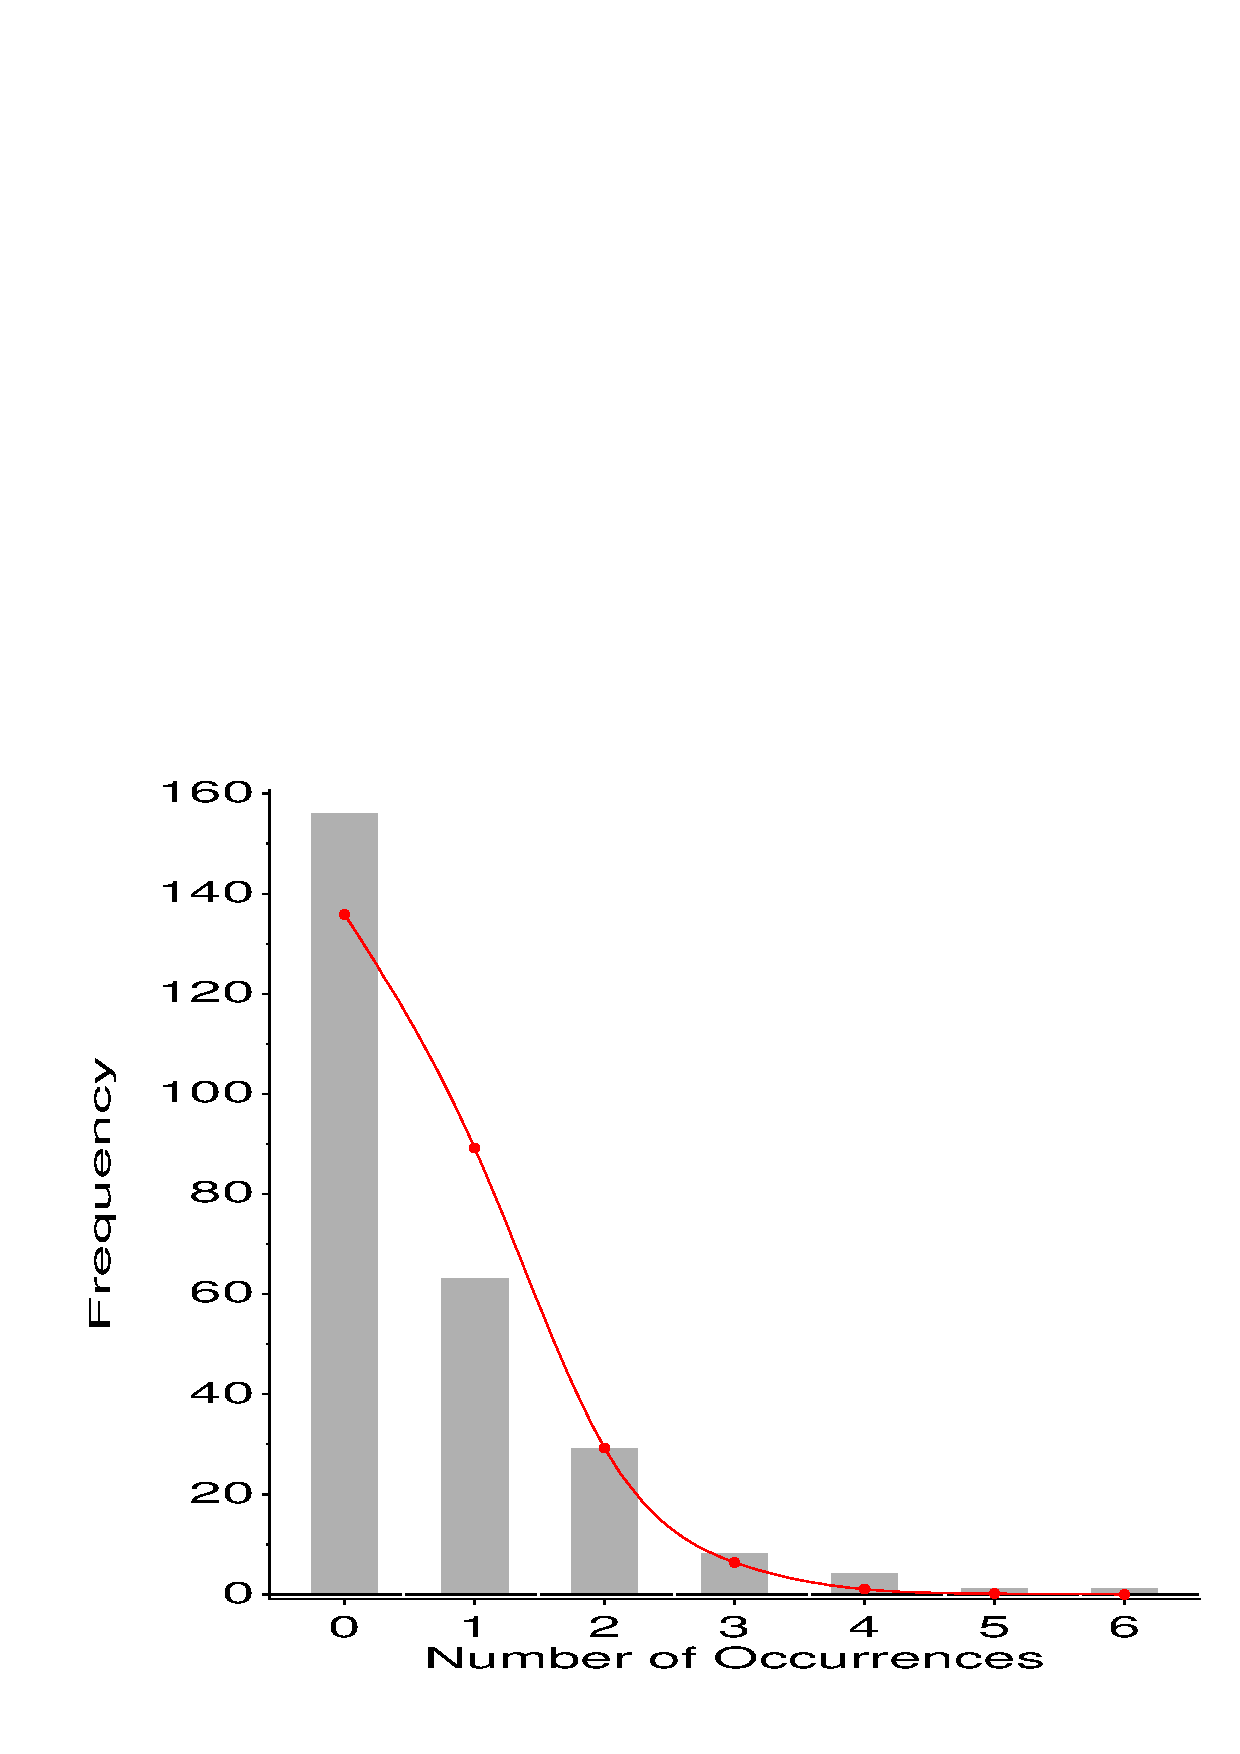
\includegraphics{madfit1}\graphicsfile{ch2/fig/madfit1.eps}{}
 }
 \subfigure[Rootogram]{\label{fig:madfit2}%
  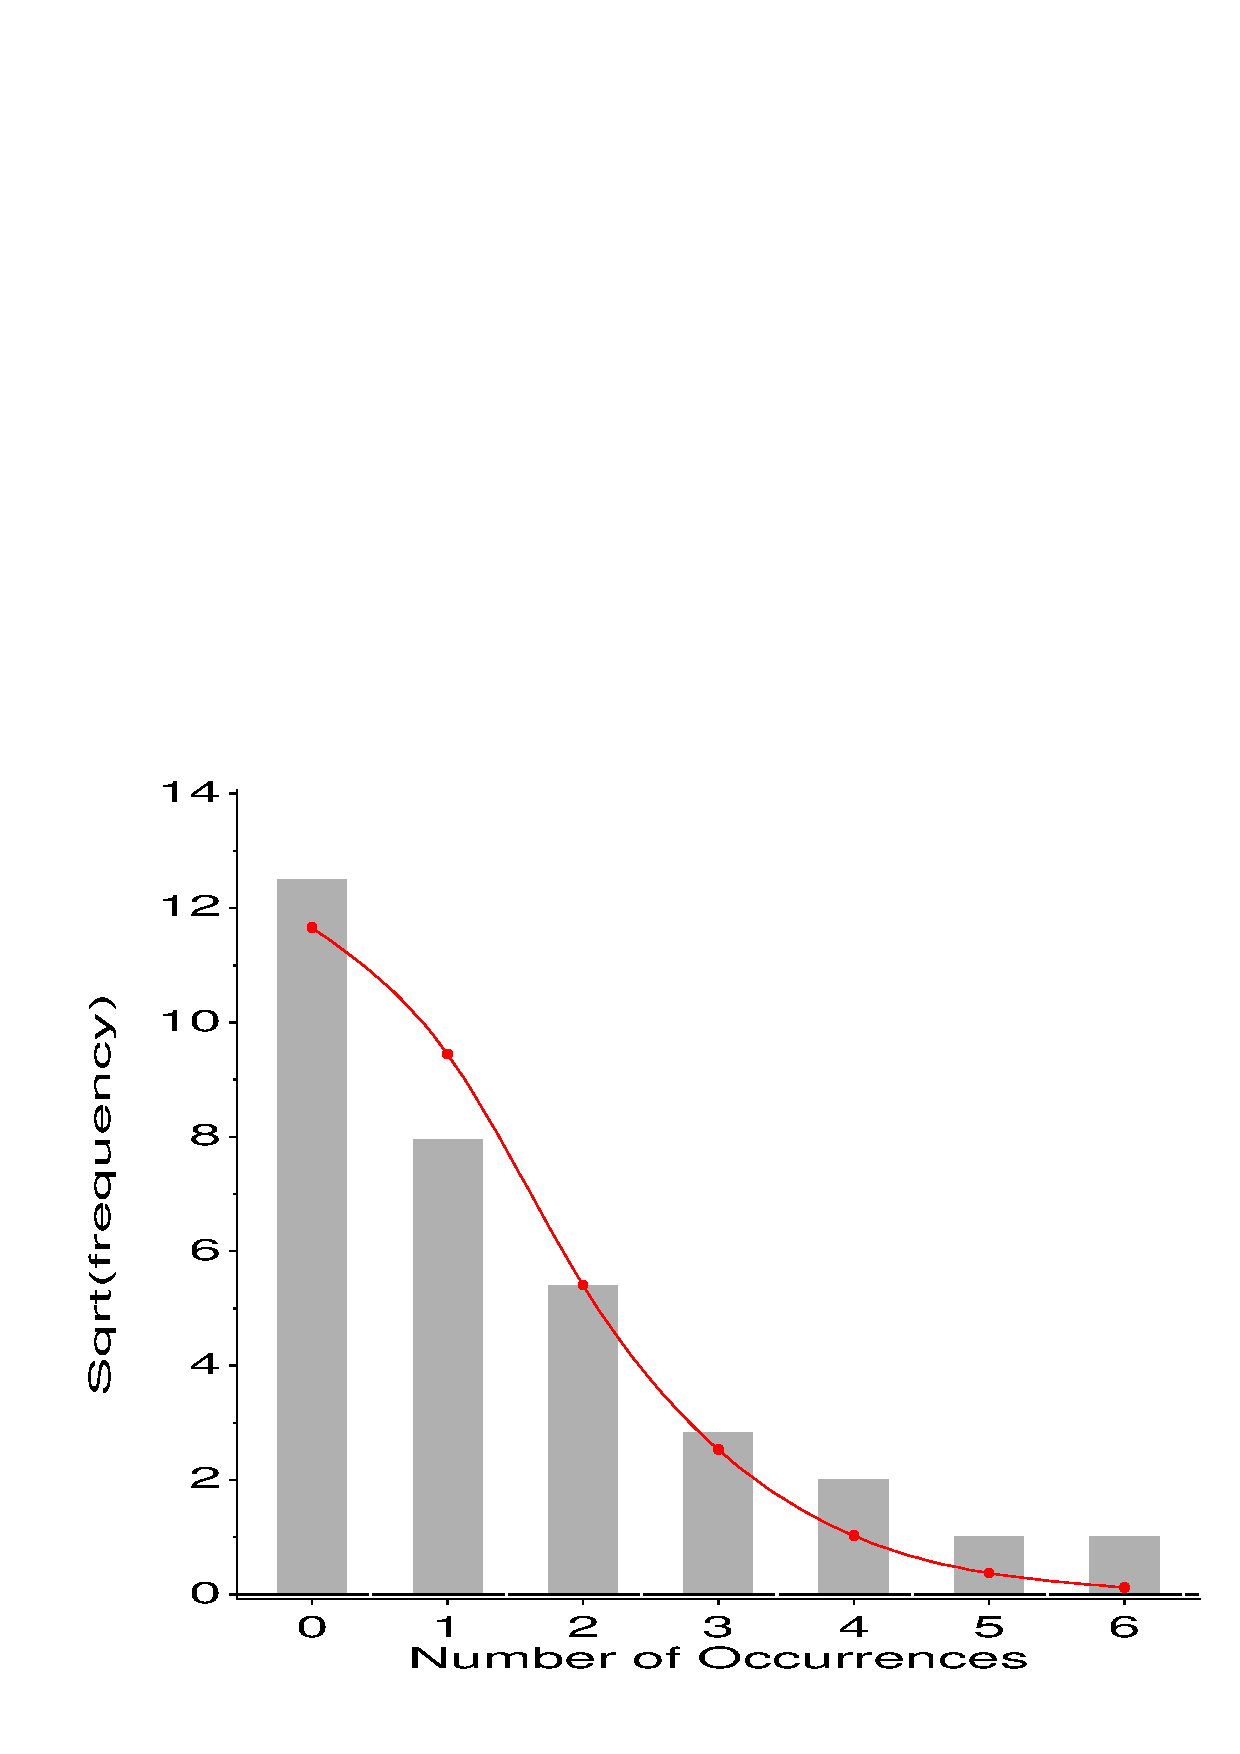
\includegraphics{madfit2}\graphicsfile{ch2/fig/madfit2.eps}{}
 }
 \subfigure[Hanging rootogram]{\label{fig:madfit3}%
  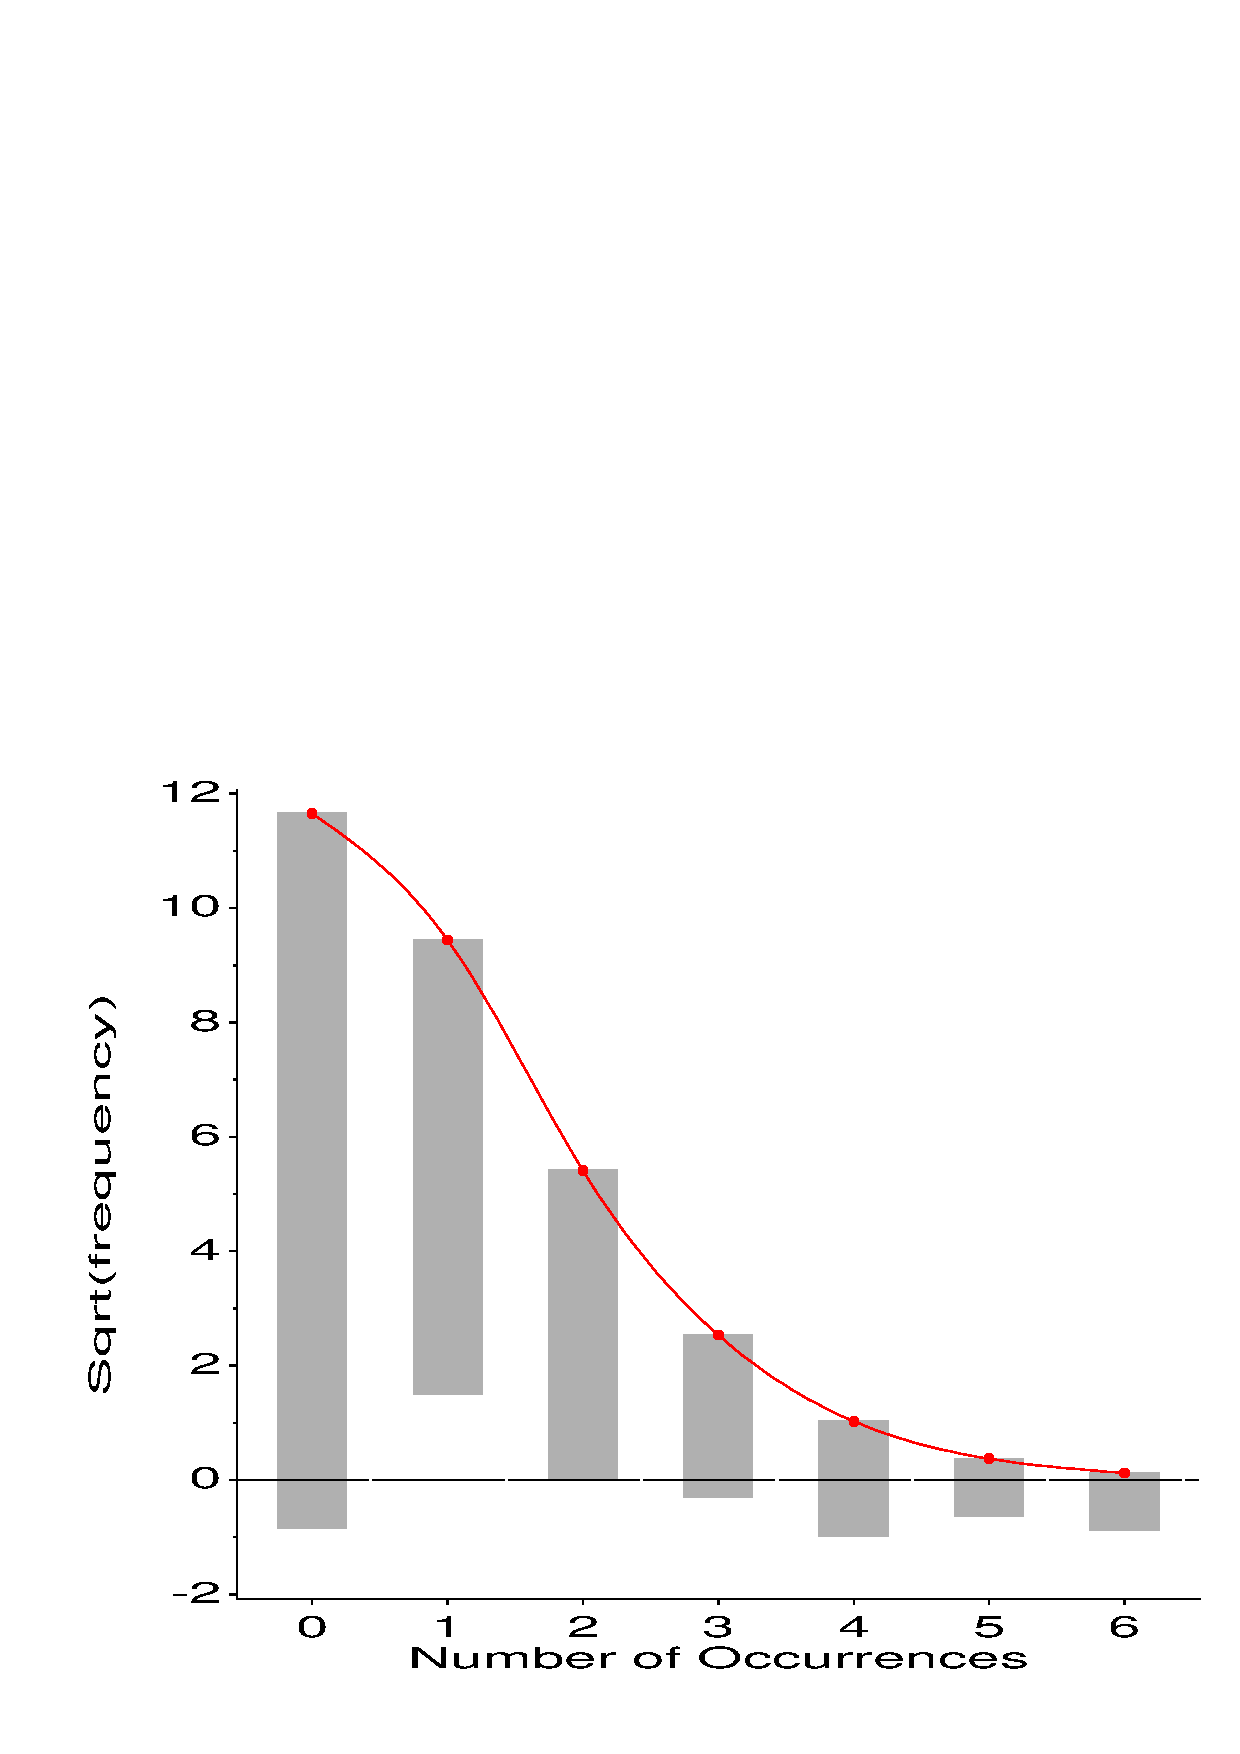
\includegraphics{madfit3}\graphicsfile{ch2/fig/madfit3.eps}{}
 }
 \subfigure[Deviation rootogram]{\label{fig:madfit4}%
  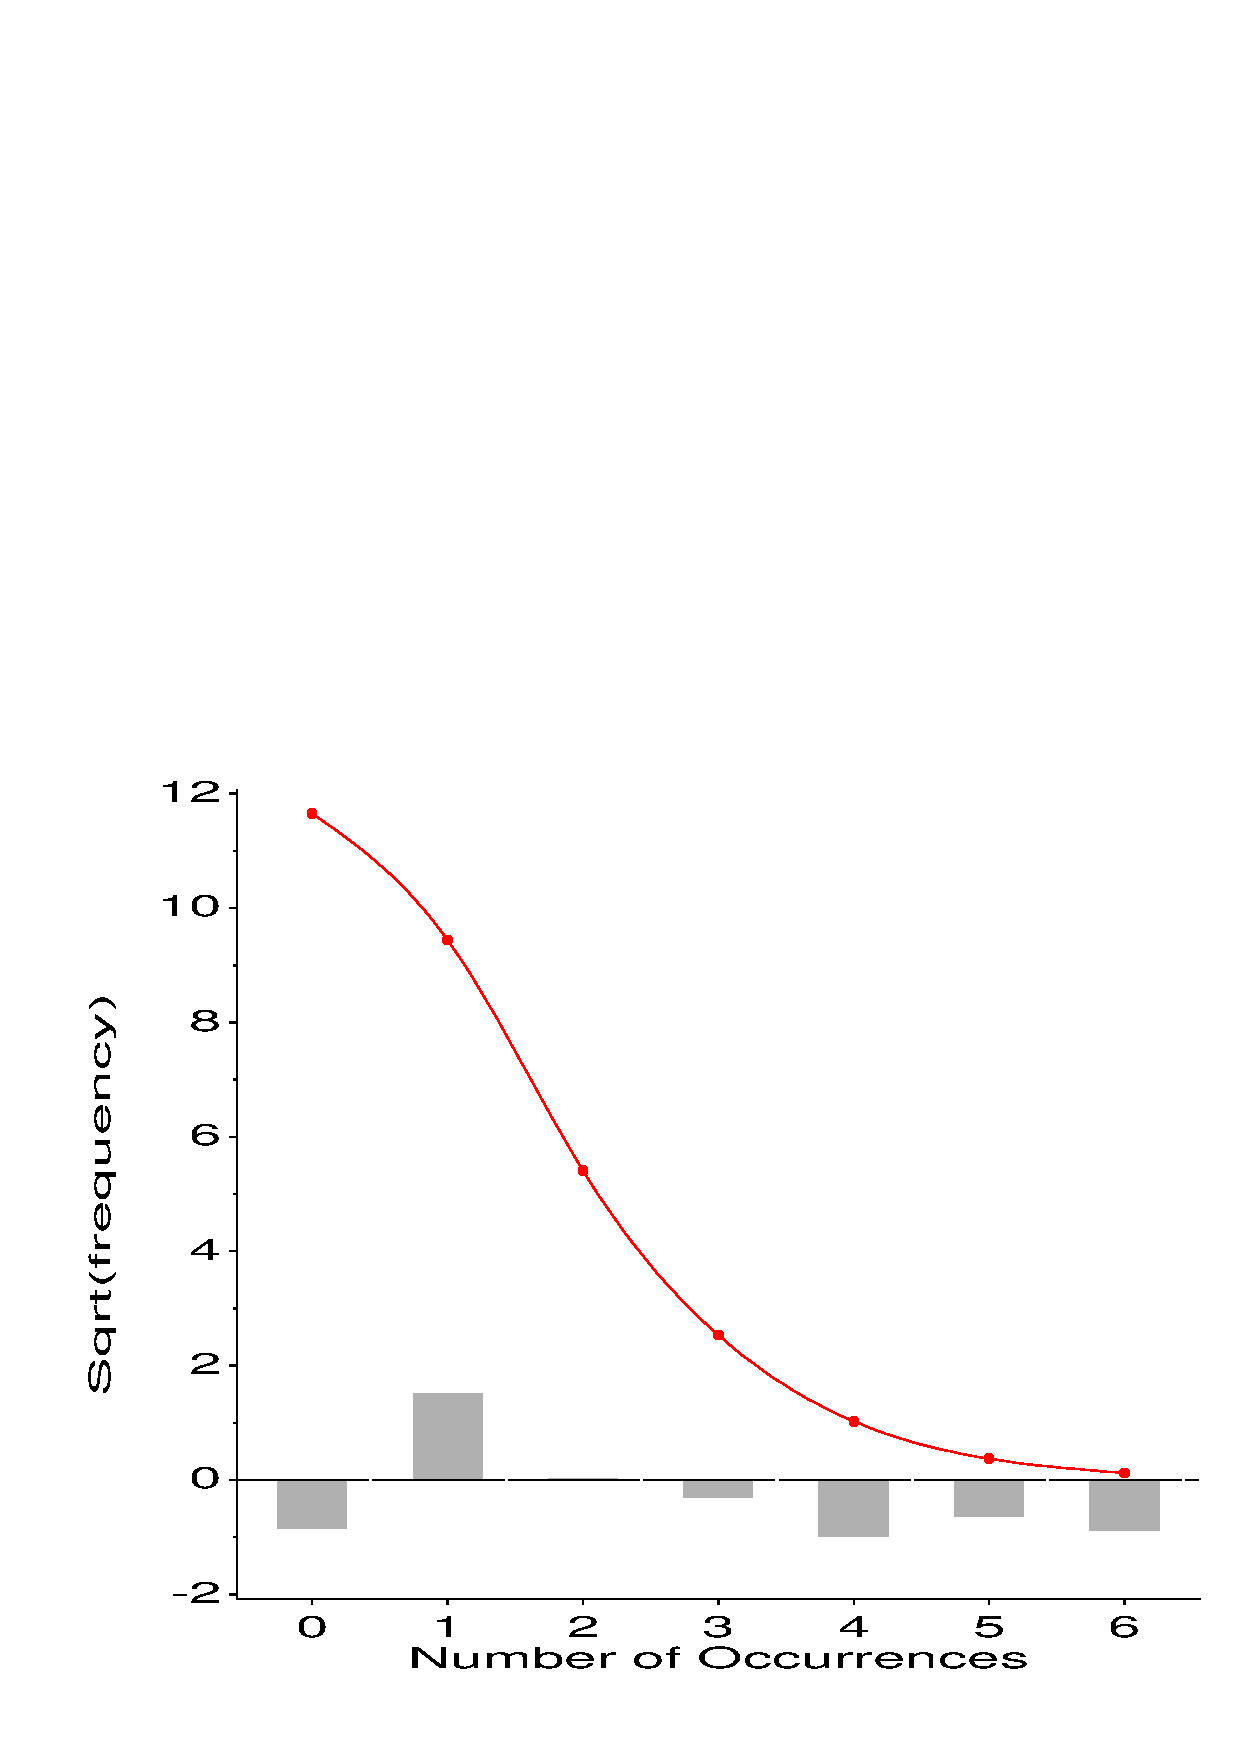
\includegraphics{madfit4}\graphicsfile{ch2/fig/madfit4.eps}{}
 }
 \end{subfigmatrix}
 \caption[Plots of observed and fitted frequencies]{Plots of observed and fitted frequencies
 for the Federalist Papers data, Poisson model.  Each panel shows the fitted frequencies as a smooth
 curve and observed frequencies as a bar.  Panel (a) raw frequencies;
 panels (b)-(d) on a square-root scale, to emphasize smaller frequencies.  Panel (c) is a hanging rootogram, where observed - fitted differences can be judged relative to the horizontal line. Panel (d) shows only the difference between the observed and fi

tted frequency.}\label{fig:madfit}
\end{figure}


\subsection{The \macro{ROOTGRAM}}\label{discrete-root}
The \macro{ROOTGRAM} (\macref{mac:rootgram}) displays observed and fitted frequencies
for a \Dset\ in any of the forms shown in \figref{fig:madfit}.
The input \Dset\ is usually of the form of the output
\texttt{OUT=} \Dset\ produced by the \macro{GOODFIT}.

\begin{Example}[federalist2]{Federalist papers}
We have seen that the negative binomial produces a better fit to the
Federalist Papers data.  The hanging rootogram (\figref{fig:madfit5}),
produced by the statements below, is characteristic of a decent fit.
\begin{listing}
%include catdata(madison);
%goodfit(data=madison, var=count, freq=blocks, dist=negbin, out=fit2);
%rootgram(data=fit2, var=count, obs=blocks, btype=dev);
\end{listing}
%\begin{figure}
%\fig{madfit5.eps}{scale=.7}{madfit5}{Hanging rootogram for the Federalist Papers data, Negative binomial model}
\fig{madfit5}{scale=.7}{Hanging rootogram for the Federalist Papers data, Negative binomial model}
%\end{figure}
\end{Example}


\begin{Example}[saxony1]{Families in Saxony}
Geissler
(cited in \citet{SokalRholf:69}
and \citet{Lindsey:95})
tabulated a huge \Dset\ on sex distributions in families in Saxony
in the 19th century.  Included were $N=6115$ families with $n=12$ children,
which might reasonably be expected to follow a Bin(12,$p$) distribution.
The data are input and fit as shown below.
%% input: /users/faculty/friendly/sasuser/catdata/saxony.sas
%% last modified: 08-Jan-98  9:29
\begin{listing}
title 'Number of males in 6115 families in Saxony';
data saxony;
   do males = 0 to 12;
      input families @;
      output;
      end;
   label males='Number of males'
      families='Number of families';
datalines;
3  24  104  286  670  1033  1343 1112  829  478  181  45  7
;

%goodfit(data=saxony, var=males, freq=families, dist=binomial);

title;
%rootgram(data=fit, var=males, obs=families, exp=exp);
\end{listing}


The fitted distribution, using the estimated proportion of males,
$p = .5192$ is shown in \outref{out:saxony.1};
the goodness of fit tests shown in \outref{out:saxony.2}
indicate that the fit of the Binomial is not good.
The hanging rootogram in \figref{fig:saxony} shows why---%
there is a systematic pattern of deviations from the Binomial,
which produces fitted frequencies too high in the middle and too small
in the tails.
The lack of fit might be ascribed to violations of the assumptions---%
a constant probability of a male birth over a long time span
is a good possibility.
\footnote{\citet[p. 131]{Lindsey:95}
fits a double binomial model with one extra parameter,
and achieves a much better fit, but this too
shows significant lack of fit, not surprising considering the
enormous sample size.}
\begin{Output}
\caption{Fit of the Binomial($12, p$) to the Families in Saxony data: Observed and fitted frequencies}\label{out:saxony.1}
\small
\verbatiminput{ch2/out/saxony.1}
\end{Output}
\begin{Output}
\caption{Fit of the Binomial($12, p$) to the Families in Saxiony data: Goodness of fit tests}\label{out:saxony.2}
\small
\verbatiminput{ch2/out/saxony.2}
\end{Output}

\begin{figure}[htb]
  \centering
  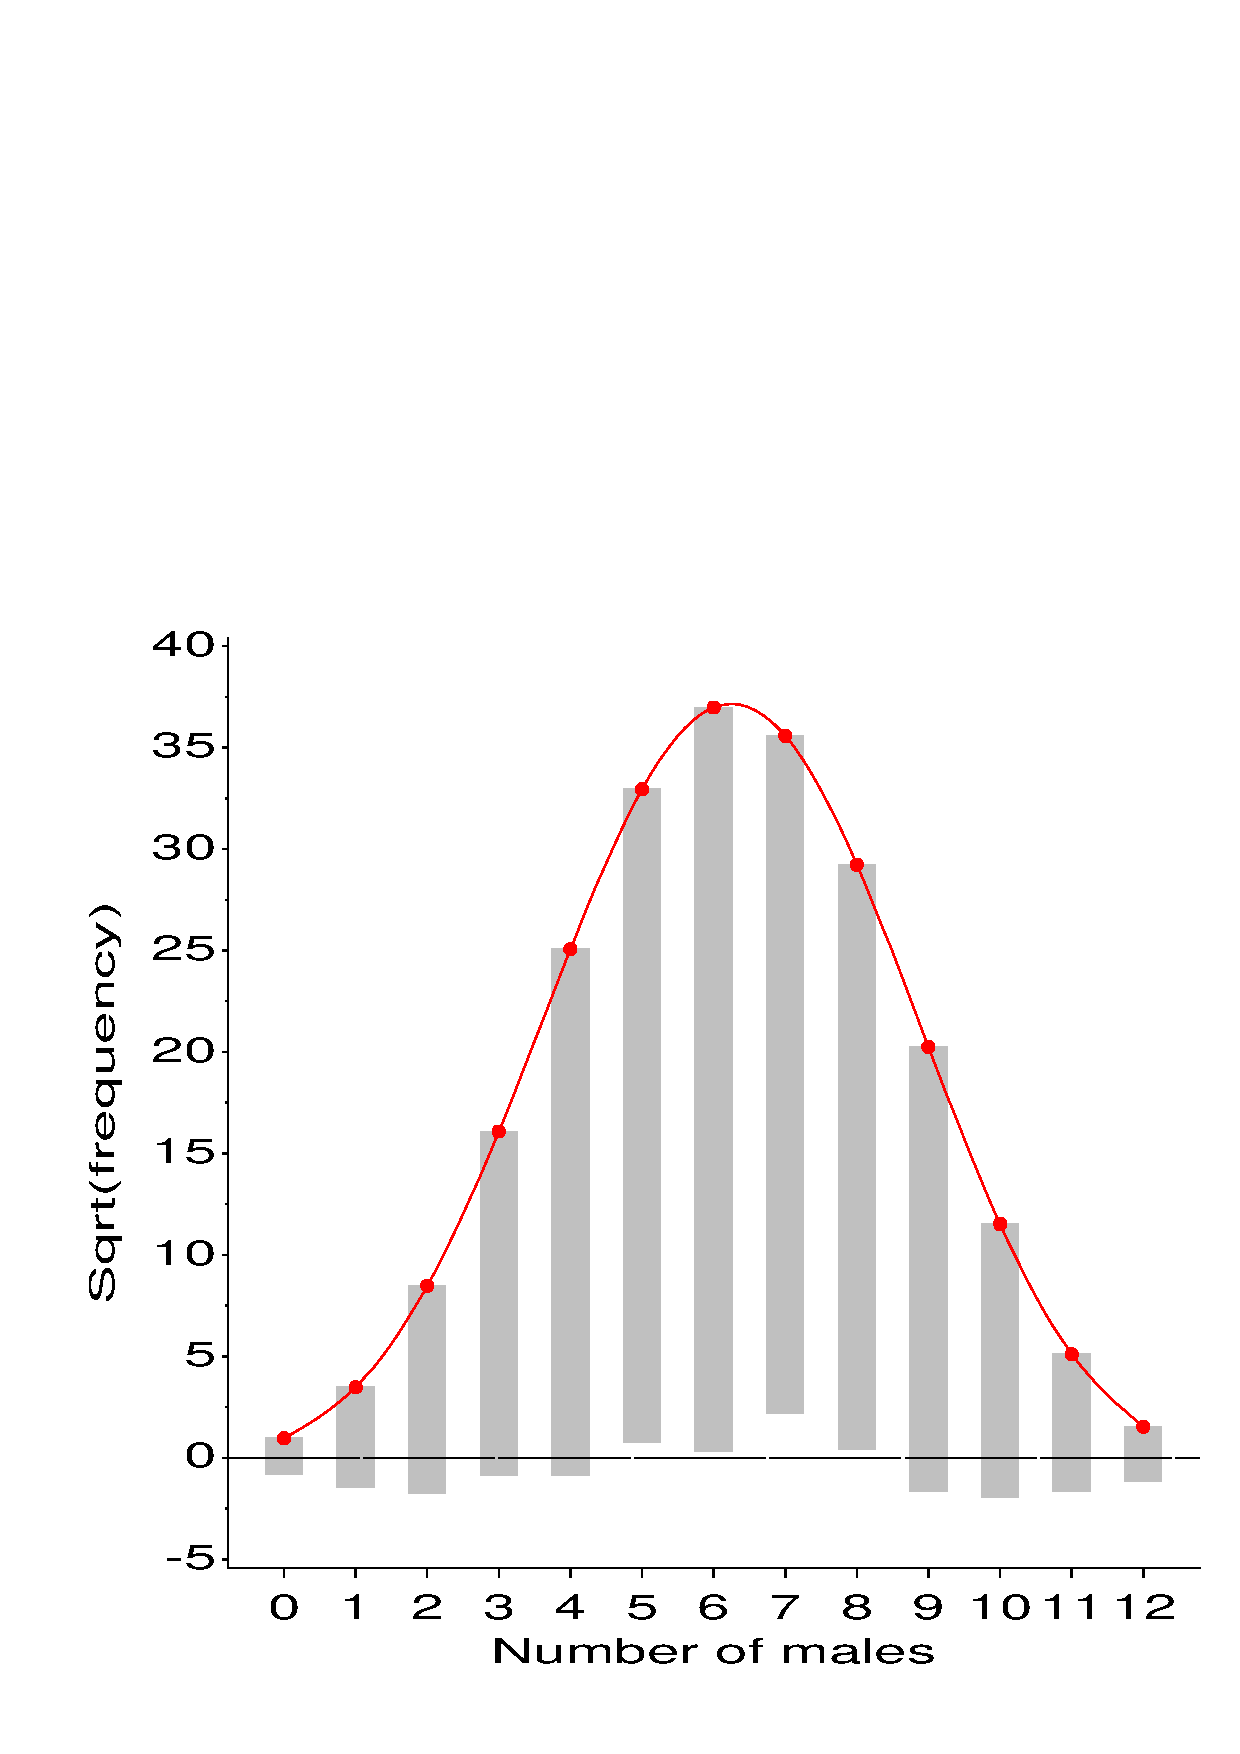
\includegraphics[scale=.5]{saxony}\graphicsfile{ch2/fig/saxony.eps}{}
  \caption[Hanging rootogram for Saxony families, Binomial model]{Hanging rootogram for Saxony families, Binomial($12, p$) model.
The systematic pattern of deviations shows that the Binomial model is not completely adequate for these data.}\label{fig:saxony}
\end{figure}
\end{Example}


\subsection{Maximum likelihood estimation}
\secref{sec:discrete-distrib} described the common discrete distributions,
their probability functions, and sample estimates.
Here we consider the general case.
Suppose we have a multinomial sample of
$K$ ``groups'', with frequencies of $n_k$ in group
$k$, and $\sum_k n_k = N$.
Suppose further that we have a probability model which specifies
the probability, \( \pi_k (\vec{\theta}), \: k = 1, 2, \dots ,  K \),
of an observation in group $k$, where $\vec{\theta}$ is a vector
of $s \geq 0$ parameters of the distribution
and $\sum_k \pi_k (\vec{\theta}) = 1$.

The likelihood, $\mathcal{L}$, is the probability of the data as
a function of the parameters,

\begin{equation*}
  \mathcal{L}(\vec{\theta}) = n ! \prod_{k=1}^K \frac{\pi_k (\vec{\theta})^{n_k}}{n_k !}
\end{equation*}

We can determine the value(s) of $\vec{\theta}$ which maximize $\mathcal{L}$
by maximizing the log-likelihood,

\begin{equation}\label{eq:loglikelihood}
 \ell(\vec{\theta}) \equiv
 \log \mathcal{L}(\vec{\theta}) = \log n ! +
  \sum_{k=1}^K n_k \log \pi_k (\vec{\theta}) - \sum_{k=1}^K \log n_k !
\end{equation}
The maximum likelihood estimate (MLE) of $\vec{\theta}$ will be
the value $\hat{\vec{\theta}}$ which is the solution of the
estimating equations
\begin{equation*}
\frac{\partial \log \mathcal{L}(\vec{\theta})}{\partial \vec{\theta}_i} = 0
\quad\quad i=1, 2, \dots s
\end{equation*}

For example, for the geometric distribution with probability
function \eqref{eq:geomf}, the log-likelihood is
\begin{equation*}
 \ell(\vec{\theta})   = n \log \theta +
  \sum_{k=1}^K (n_k - 1) \log (1-\theta)
\end{equation*}
which gives the estimating equation,
\begin{equation*}
\frac{\partial \ell(\theta)}{\partial \theta} =
\frac{(\sum_k n_k) - n}{1-\theta} + \frac{n}{\theta} = 0
\end{equation*}
whose solution is $\hat{\theta} = 1/\bar{k}$.  The fitted probabilities
under the geometric model
are then $\pi_k (\hat{\theta}) = (1 - \hat{\theta})^{k-1} \hat{\theta}$.

Having found the maximum likelihood estimate of the parameters, the
likelihood ratio
goodness-of-fit \GSQ{} statistic compares the maximized value of the
log-likelihood to the maximized log-likelihood of an unrestricted model
where the probabilities are only constrained so that $\sum_k \pi_k =1$.
In this case, there are $s=0$ parameters, and we symbolize the log-likelihood
by $ \ell(\theta_0) \equiv \ell(\vec{\pi})$.  For a multinomial sample this is

\begin{equation}\label{eq:loglikelihood0}
 \ell(\vec{\theta}_0)  = \log n ! +
  \sum_{k=1}^K n_k \log \pi_k  - \sum_{k=1}^K \log n_k !
\end{equation}
Maximizing \eqref{eq:loglikelihood0} subject to $\sum_k \pi_k =1$
gives $\hat{\pi}_k = n_k / N$.
The likelihood ratio statistic is

\begin{equation}\label{eq:likeratio}
 G^2 = -2 \log \left[
 \frac{\mathcal{L}(\vec{\theta}_0)}{\mathcal{L}(\vec{\theta})}
 \right]
 = 2 [ \ell(\vec{\theta}) - \ell(\vec{\theta}_0) ]
 = 2 \sum_{k=1}^{K} n_k \log \left( \frac{n_k}{N \pi_k (\hat{\theta}) } \right)
\end{equation}
which follows an asymptotic chi-square distribution with $K-1-s$ degrees
of freedom.


\subsection{Fitting discrete distributions as \loglin\ models}
In \secref{sec:pwrseries}, I described how the common discrete distributions
are all members of the general power series family.
Another general family of distributions---the exponential family---%
includes most of the common continuous distributions:
the normal, gamma, exponential, and others,
and is the basis of the class of generalized linear models fit
by \PROC{GENMOD}.

\citet{LindseyMersch:92}, \citet[6.1]{Lindsey:95} have shown how various discrete
(and continuous)
distributions can be fit to frequency data using Poisson \loglin{} models
available in \PROC{GENMOD}.  The uniform, geometric, binomial, and the
Poisson distributions may all be fit easily in this way.
A clear advantage is that this method gives estimated standard errors for the
distribution parameters as well as estimated confidence intervals
for fitted probabilities.

The essential idea is that, for frequency data, any distribution in the
exponential family may be represented by a linear model for the logarithm
of the cell frequency, with a Poisson distribution for errors,
otherwise known as a ``Poisson \loglin\ regression model''.
These have the form
\begin{equation*}
\log (N \pi_k) = \textrm{ offset } + \beta_0 + \vec{\beta}\trans \vec{S}(k)
 \comma
\end{equation*}
where $\vec{S}(k)$ is a vector of zero or more sufficient statistics for the
canonical parameters of the exponential family distribution,
and the offset term is a value which does not depend on the
parameters.  \tabref{tab:expfamily} shows the sufficient statistics and
offsets for several discrete distributions.
See \citet{LindseyMersch:92} for further details, and definitions
for the double-binomial distribution.

\begin{table}[tb]
 \caption{Poisson \loglin\ representations for some discrete distributions}\label{tab:expfamily}
 \begin{center}
{\renewcommand{\arraystretch}{1.2}
 \begin{tabular}{lll}
  \hline
  \tableheader
  Distribution & Sufficient statistics & Offset \\
  \hline
  Geometric & $k$ \\
  Poisson & $k$ & $-\log(k!)$ \\
  Binomial & $k$ & $\log{\binom{n}{k}}$ \\
  Double binomial & $k, k \log(k) + (n-k) \log(n-k)$ & $\log{\binom{n}{k}}$ \\
  \hline
 \end{tabular}
}
 \end{center}
\end{table}


\begin{Example}[saxony2]{Families in Saxony}
The binomial distribution and the double binomial can both be fit to frequency data as a Poisson
regression using $\log \binom{n}{k}$ as an offset.
We only display results for the binomial model.
\begin{listing}
*-- calculate offset variables for binomial and double binomial;
data saxony;
   set saxony;
   logkn = log( gamma(12+1) / (gamma(males+1) * gamma(12-males+1)) );
   if 0 < males < 12
      then ylogity = -males * log(males/(12-males));
      else ylogity = 0;

   *-- fit binomial (12,p);
proc genmod data=saxony;
   model families = males /
      dist=poisson offset=logkn obstats ;

   *-- fit double binomial (12,p, psi);
proc genmod data=saxony;
   model families = males ylogity /
      dist=poisson offset=logkn obstats ;
\end{listing}
The goodness of fit tests shown in \outref{out:saxony2.1}
are equivalent to those calculated directly by the
\macro{GOODFIT} in \outref{out:saxony.2}.
The parameter estimate for \texttt{MALES}, $\beta_1 = 0.0769$
is actually estimating the logit of $p$, $\log p / (1-p)$,
so the inverse transformation gives
$\hat{p} = \frac{\exp (\beta_1)}{1 + \exp (\beta_1)} = 0.5192$,
as we had before.
The fitted frequencies (shown in \outref{out:saxony2.2}), given by the \opt{OBSTATS}{GENMOD}
on the \stmt{MODEL}{GENMOD} are the same as those
in \outref{out:saxony.1}.
The standard error for \texttt{MALES}, $s_{\beta_1} = 0.0074$
could also be transformed back to the probability scale in the same
way.
\begin{Output}
\caption{Fit of the Binomial($12, p$) to the Families in Saxony data: Goodness of fit tests}\label{out:saxony2.1}
\small
\verbatiminput{ch2/out/saxony2.1}
\end{Output}
\begin{Output}
\caption{Fit of the Binomial($12, p$) to the Families in Saxony data: Observed and fitted frequencies}\label{out:saxony2.2}
\small
\verbatiminput{ch2/out/saxony2.2}
\end{Output}
\end{Example}

